\subsection{Methods}
\frame{
  \frametitle{B-Splines for Surface Representation}
  \textit{Splines}: piecewise polynomial function of degree <$d$.

  \textit{B(asis)-Splines}: Specific choice of finite-support splines for basis.

      \begin{figure}[h!]
        \centering
        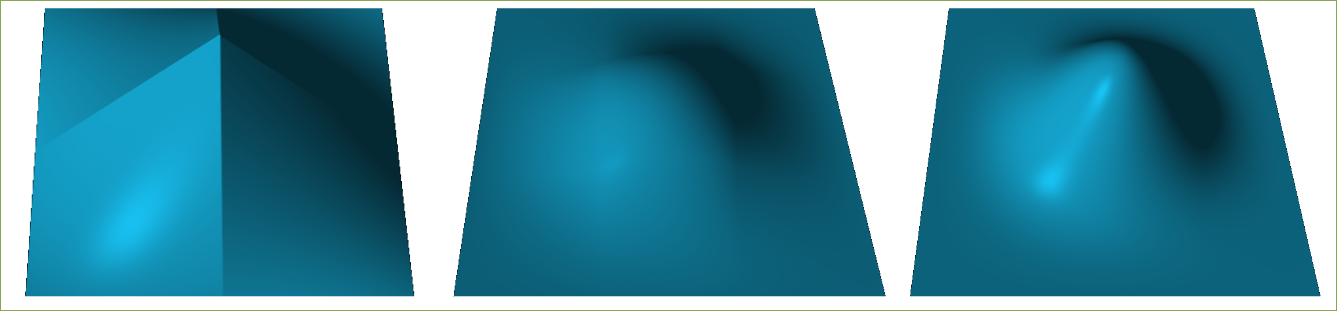
\includegraphics[width=.4\textwidth]{figures/degrees.png}
      \end{figure}

      \vspace{-1em}

      \begin{columns}
        \column{.5\textwidth}

      \begin{figure}[h!]
        \centering
        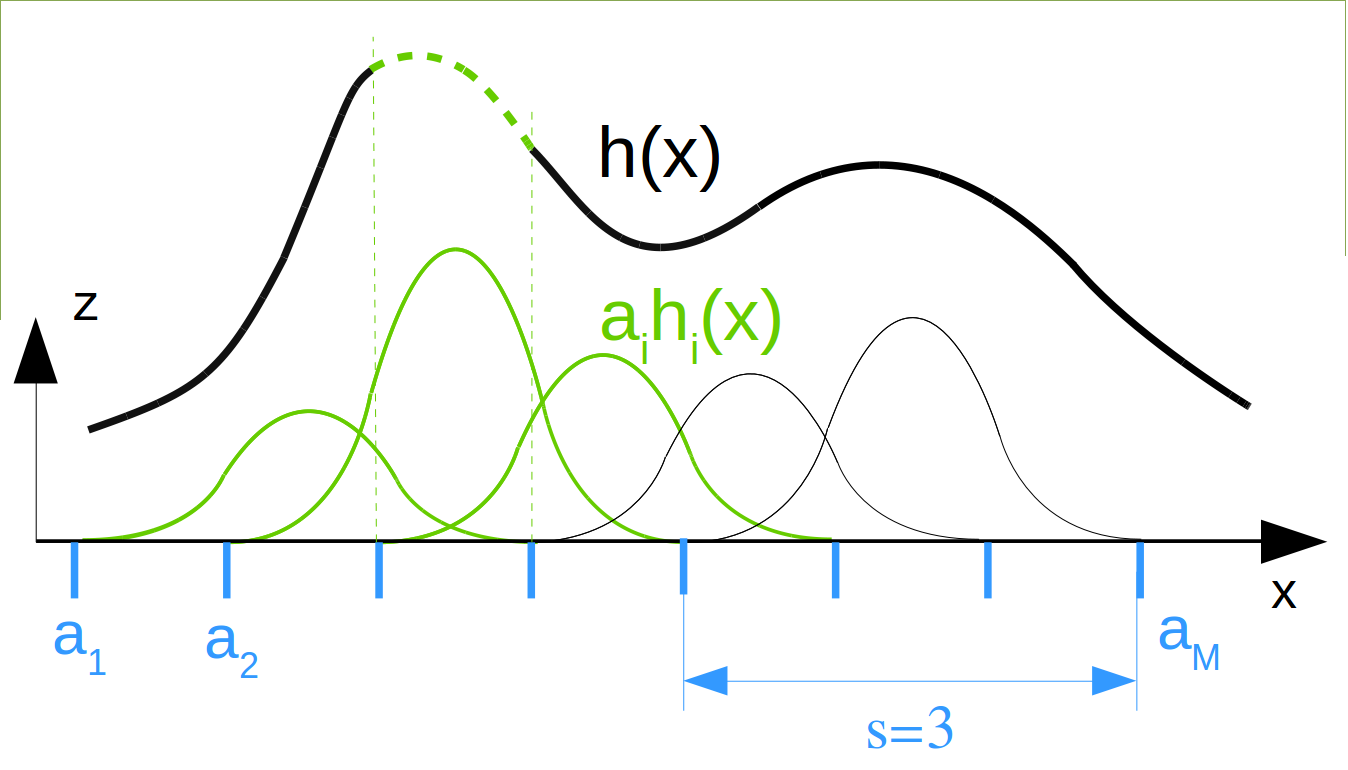
\includegraphics[width=.9\linewidth]{figures/spline.png}
        % \caption{Quadratic spline basis functions and resulting spline surface in
        % 1D.}
        \label{fig:splines}
      \end{figure}

     % with $k$ the index of the first non-zero spline function for $x_j$ and 
     % $s$ is the support of the spline function ($s = d + 1$).

        \column{.5\textwidth}
     \begin{align*}
       h(x_j) &= \sum_{i=0}^{\g{M}}\gi{a} h_i(x_j)\\
       &= \sum_{i=k}^{k + \g{s}} \gi{a} h_i(x_j)\text{, for } j = 1 \ldots \g{N}
       \label{test}
     \end{align*}
    \end{columns}
}

\frame{
  \frametitle{Stereo Camera Setup}

  \begin{columns}
    \column{.5\linewidth}

  \begin{figure}[h!]
    \centering
    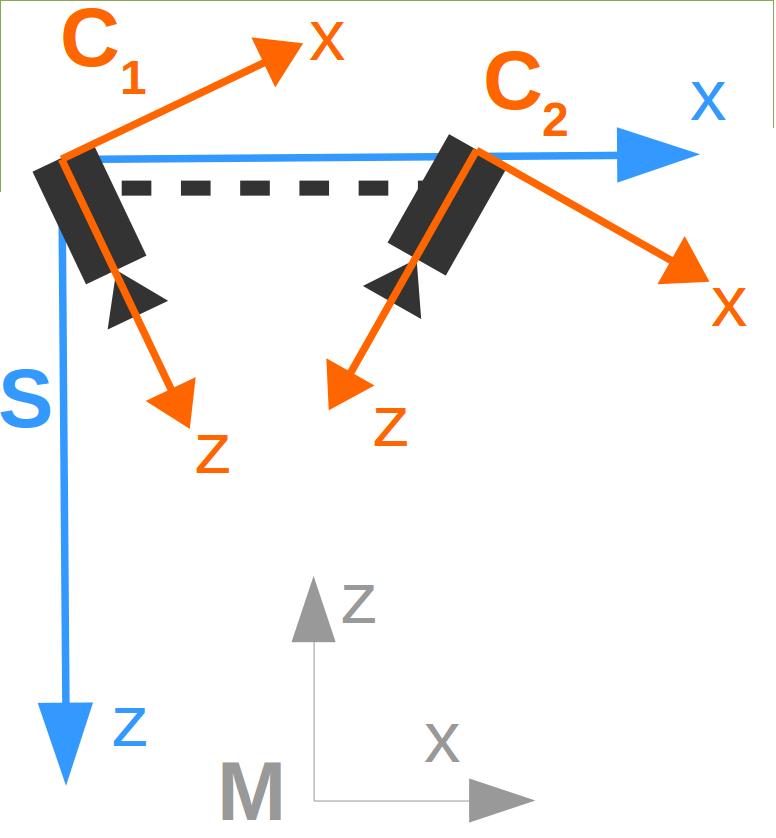
\includegraphics[width=.6\linewidth]{figures/camerasetup.png}
  \end{figure}
    
    \column{.5\linewidth}

  Camera poses described by \g{mrmc} and \g{ccm} for $k = 1, 2$ or 
  \begin{align*}
    \g{xi}_{C_k} &:= \begin{bmatrix} \g{mrmc}, \g{phic} \end{bmatrix}^T \\
    \g{xi}_S &:= \begin{bmatrix} \g{mrms}, \g{phis} \end{bmatrix}^T
  \end{align*}

  with \g{phic}, \g{phis} $\in\mathbb{R}^3$ \cite{Primer}
  %are the coordinate tuples associated with the relative orientation of the respective coordinate frames. 
\end{columns}

\vspace{1em}

Relative position of $\{ \g{xi}_{C_1}, \g{xi}_{C_2}, \g{xi}_S \}$ stays fixed.

}

\frame{
  \frametitle{Photometric errors for mapping}

  \begin{columns}
    \column{0.35\linewidth}

    \vspace{-1em}
  
    \begin{figure}[h!]
      \centering
      \begin{subfigure}{0.3\linewidth}
        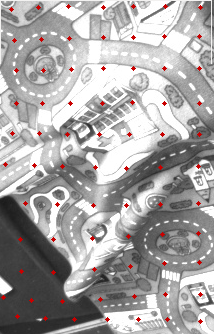
\includegraphics[height=1.5\textwidth]{figures/pixels1_strip.png}
      \end{subfigure}
      \begin{subfigure}{0.3\linewidth}
        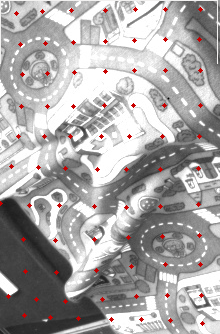
\includegraphics[height=1.5\textwidth]{figures/pixels2_strip.png}
      \end{subfigure}
      \begin{subfigure}{0.3\linewidth}
        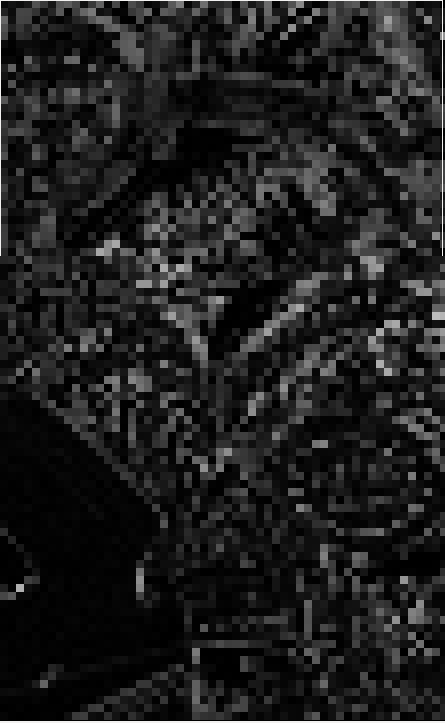
\includegraphics[height=1.5\textwidth]{figures/residuals_strip.png}
      \end{subfigure}
      \label{fig:pixels}
    \end{figure}

    \vspace{-1em}

    \begin{figure}[h!]
      \centering
      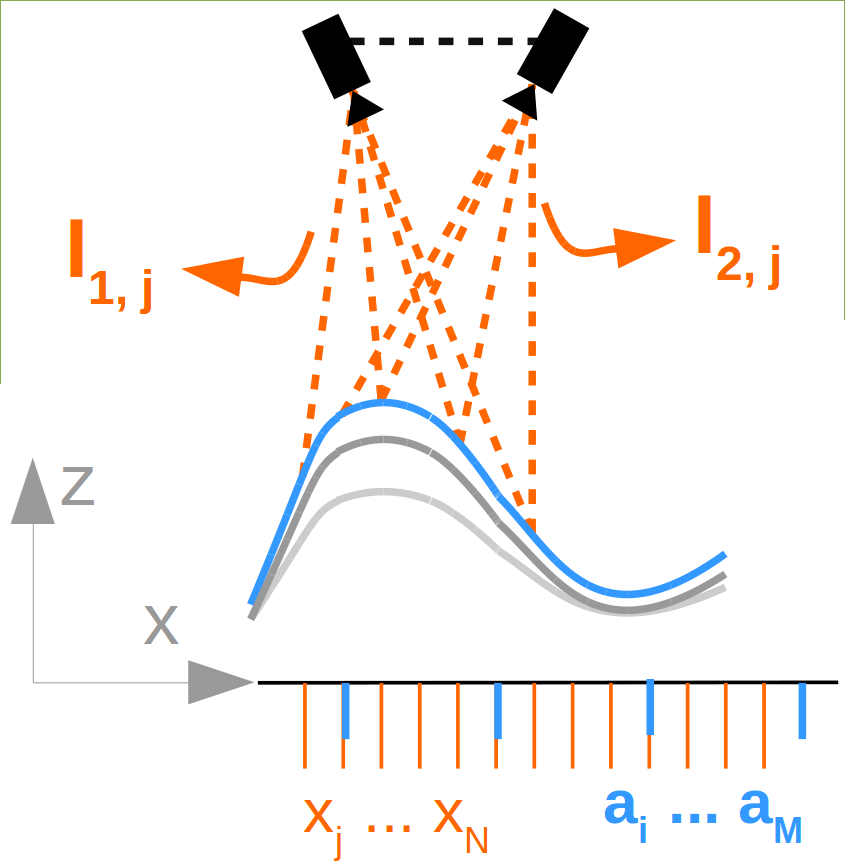
\includegraphics[width=.8\linewidth]{figures/mapping.png}
      \label{fig:photometric}
    \end{figure}

  \column{0.64\linewidth}

    \only<1-1>{

    Photometric error of grid point $x_j, y_j$:

    %TODO CONTINUE HERE!
    \begin{equation*}
      r_j = I_1(\vc u_{j,1}(\g{a})) - I_2(\vc u_{j,2}) \text{ ,}
      \label{eq:photometric}
    \end{equation*}

    with $I_1$, $I_2$ interpolated intensities at the locations $\vc u_{j,k}$ in camera
    $k = 1$ and $k=2$.

    \vspace{-1em}

  \begin{align*}
    \vc u_{j,k} &= \vc K_k D_k(\g{Tk}(\g{mrmx}))) \\
    \g{Tk}(\g{mrmx}) &= \g{pi}(\g{ccm} (\g{mrmx} - \g{mrmc})) \hspace{1em} 
    \label{eq:pixel}
  \end{align*}

  3D point given by spline map:

  \begin{equation*}
    \g{mrmx} = \begin{bmatrix} x_j, y_j, h(x_j, y_j) \end{bmatrix} ^T
  \end{equation*}
}
    \only<2-2>{

  \begin{equation*}
    \g{Jrs} = \frac{\partial \vc r(\g{a})}{\partial\g{a}} \in\mathbb{R}^{\g{N}x\g{M}}
  \end{equation*}
       
  \begin{align*} 
    \g{Jrs} &= (\vc J_{pixel, 1} \vc J_{camera, 1}(\g{mrmx}) \\
    &- \vc J_{pixel, 2} \vc J_{camera, 2}(\g{mrmx})) \vc J_{splines} \text{ .}
  \end{align*}

  \begin{align*}
    \vc J_{pixel, k} &= \frac{\partial I_k(\vc u_{k})}{\partial \vc{\tilde{u}}_{k}},
    \hspace{1em}
    \vc J_{camera, k}(\g{mrmx}) = \frac{\partial
      \vc{\tilde{u}}_{k}}{\partial \g{mrmx}} \\
    \vc J_{splines} &= \frac{\partial \g{mrmx}}{\partial \g{a}}
  \end{align*}

  }
  \end{columns}
}

\frame{
  \frametitle{Optimization problem for mapping}

  \begin{align*}
    \giii{a} &= \argmin{\g{a}\in\mathbb{R}^{\g{M}}} f(\g{a}) = \argmin{\g{a}\in\mathbb{R}^{\g{M}}} \frac{1}{2} (\sum_{j =
             0}^{\g{N}} \textcolor{red}{w_j} r_j(\g{a})^2
    + \textcolor{blue}{\beta \g{a}^T \vc B \g{a}} 
    + \textcolor{green}{\gamma \g{a}^T \vc G \g{a}}) \text{ ,}
  \end{align*}

  with 

  \begin{itemize}
    \item \textcolor{blue}{bending} and \textcolor{green}{gradient} energy regularization terms
      and
    \item \textcolor{red}{weight} representing the average visibility of point $j$.
  \end{itemize}


  \vspace{1em}
  Solved using Gauss-Newton iterations: 

  \centering{
\begin{align*}
  \g{a}_{k+1} &= \g{a}_k + \alpha_k \mathbf p_k^{GN}\\
  \g{Jf}^T \g{Jf} \mathbf p_k^{GN} &= - \g{Jf} ^T \mathbf r_k(\g{a})
\end{align*}
}
}

\frame{
  \frametitle{Photometric errors for localization}

  \begin{columns}
    \column{0.4\linewidth}
  
    \begin{figure}[h!]
      \centering
      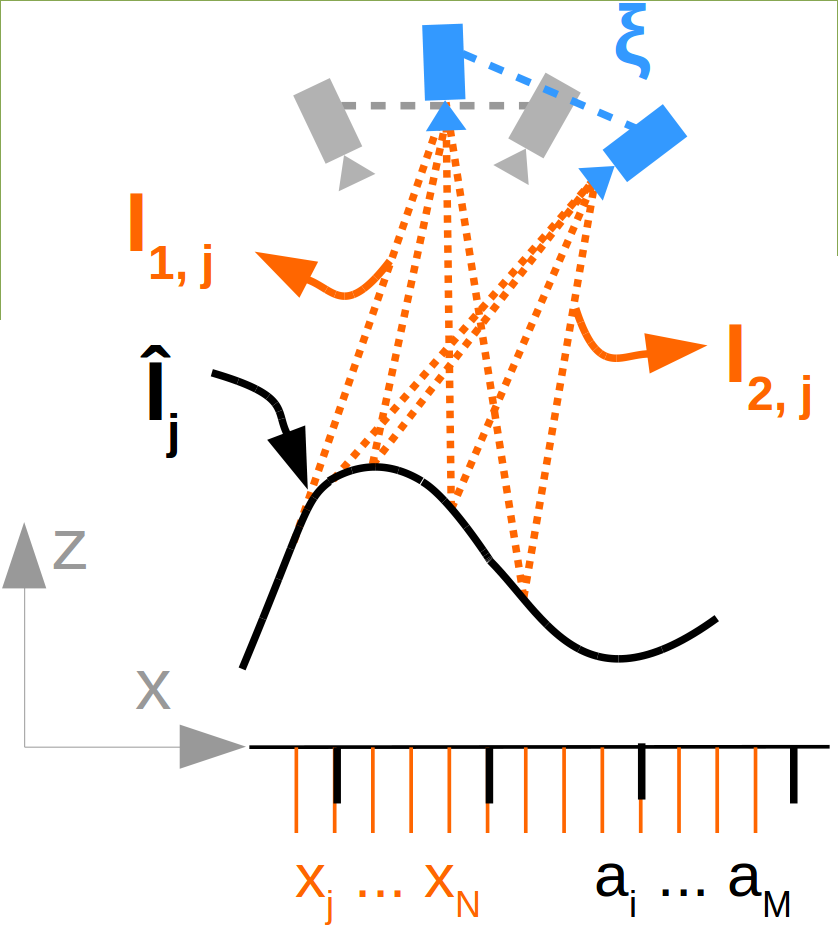
\includegraphics[width=\linewidth]{figures/localization.png}
      \label{fig:photometric}
    \end{figure}

    \column{0.6\linewidth}

    \only<1-1>{

    Photometric error of grid point $x_j, y_j$:

    \begin{align*}
      r_{j,1} &= I_1(\vc u_{j,1}) - \hat{I}(x_j, y_j) \\
      r_{j,2} &= I_2(\vc u_{j,1}) - \hat{I}(x_j, y_j) \text{ ,}
    \end{align*}

    with $I_1$, $I_2$ interpolated intensities at pixels $\vc u_{j,k}$ in camera
    $k = 1$ and $k=2$ and $\hat{I}(x_j, y_j)$ the estimated intensity from
    previous step.
    
  }
    \only<2-2>{

\begin{equation*}
  \g{Jrp} = \frac{\partial \vc r(\g{xi})}{\partial\g{xi}} \in\mathbb{R}^{\g{N}x6}
\end{equation*}
     
    \begin{align*} 
      \g{Jrp} &= \vc J_{pixel} \vc J_{camera}(\g{xi})
    \end{align*}

    with 

    \begin{align*}
      \vc J_{pixel} = \frac{\partial I(\vc u)}{\partial \vc{\tilde{u}}},
      \hspace{0.5em}
      \vc J_{camera}(\g{xi}) = \frac{\partial \vc{\tilde{u}}}{\partial \g{xi}}
    \end{align*}
}
\end{columns}

}

\frame{
  \frametitle{Optimization problem for localization}

  \begin{equation*}
    \giii{xi} =  \argmin{\giii{xi}\in\mathbb{R}^6} \frac{1}{2} 
    \sum_{j = 0}^{\g{N}} r_j(\g{xi})^2
  \end{equation*}
  
  \vspace{1em}
  Solved using Gauss-Newton iterations: 

\begin{align*}
  \g{xi}_{k+1} &= \g{xi}_k \boxplus \alpha_k \mathbf p_k^{GN}\\
  \g{Jrp}^T \g{Jrp} \mathbf p_k^{GN} &= - \g{Jrp} ^T \mathbf r_k(\g{xi})
\end{align*}
}
